\section{Two Real Klein Gordon Fields}

Since our final goal is to describe all particles and their interactions, we can start to study a more complex model: the quantization of a system with more than one field.

The simplest generalization is the following: two real KG fields \(\psi_1\) and \(\psi_2\) with different masses \(m_1 \neq m_2\). We are assuming the fields to be free, non interacting, so we can write the Lagrangian as the sum of two independent KG Lagrangian:
\[
    \mathcal{L} = \sum_{i=1,2} \frac{1}{2}\partial_\mu \psi_i \partial^{\mu} \psi_i - \frac{m_i^2}{2}\psi_i^2.
\]
Since the lagrangian is a sum of decoupled and independently Lagrangians, we can derive the KG equation as a system of two independent equations:
\[
    \begin{dcases}
        (\Box + m_1^2) \psi_1(x) = 0; \\
        (\Box + m_2^2) \psi_2(x) = 0. \\
    \end{dcases}
\]
Following this procedure, other foundamental quantities will be defined as the sum of the corresponding quantities defined for the single scalar field: we are interested in Hamiltonian, momentum and number of particles:
\[
    H = H_1 + H_2, \quad \mathbf{P} = \mathbf{P}_1 + \mathbf{P}_2, \quad N = N_1 + N_2.
\]
Now we can use ladder operators in normal ordering to promote those quantities to operators acting on the fields:
\[
    \begin{aligned}
        \hat{H}_i & = \int \frac{\mathrm{d}^3 \mathbf{p}}{(2\pi)^3}\, \omega_{i,\,\mathbf{p}} \hat{a}^{\dagger}_{i,\,\mathbf{p}}\hat{a}_{i,\,\mathbf{p}}; \\
        \hat{P}_i & = \int \frac{\mathrm{d}^3 \mathbf{p}}{(2\pi)^3}\, \mathbf{p} \hat{a}^{\dagger}_{i,\,\mathbf{p}}\hat{a}_{i,\,\mathbf{p}};              \\
        \hat{N}_i & = \int \frac{\mathrm{d}^3 \mathbf{p}}{(2\pi)^3}\, \hat{a}^{\dagger}_{i,\,\mathbf{p}}\hat{a}_{i,\,\mathbf{p}}.
    \end{aligned}
\]
Notice how we are basically spanning all the space (with the integral over all possible momenta) and counting the particles in it, then multiplying them by the actual eigenvalue in which we are interested: \(\omega_{i,\,\mathbf{p}}\) for the energy or \(\mathbf{p}\) for the momentum. The ladder operators create or destroy a particle of mass \(m_i\) and momentum \(\mathbf{p}\) accordingly to the previous definitions:
\[
    \ket{\mathbf{p}_{(1)}} = \hat{a}^{\dagger}_{1,\,\mathbf{p}} \ket{0}, \quad \ket{\mathbf{p}_{(2)}} = \hat{a}^{\dagger}_{2,\,\mathbf{p}} \ket{0},
\]
where these particles have different masses and energies
\[
    \hat{H} \ket{\mathbf{p}_{(1)}} = \omega_{1,\,\mathbf{p}} \ket{\mathbf{p}_{(1)}}, \quad \omega_{1,\,\mathbf{p}}\neq \omega_{2,\,\mathbf{p}} \text{ since } m_1 \neq m_2;
\]
but they are degenerate as far as number of particles and momentum are concerned:
\[
    \begin{aligned}
        \hat{P} \ket{\mathbf{p}_{(i)}} & = \mathbf{p} \ket{\mathbf{p}_{(i)}}, \quad \mathbf{p}_1 = \mathbf{p}_2 = \mathbf{p}; \\
        \hat{N} \ket{\mathbf{p}_{(i)}} & = 1 \ket{\mathbf{p}_{(i)}}, \quad n=1 \text{ for both fields.}
    \end{aligned}
\]
Thus these three operators are simultaneously diagonalizable, having the same set of eigenstates (forming a complete ON basis) but different eigenvalues.

The more interesting case is when both fields share the same mass \(m_1 = m_2 = m\): what happens to the system?\footnote{We drop for now the index \(i\) on the energy \(\omega_i,\mathbf{p}\) since they are equal for both fields, but in the following refinements we will reintroduce them to avoid confusion.}
To start now we have equal eigenvalues for all the three previously considered operators.
Furthermore, if we imagine the two KG fields as two axis of a plane we can deduce a new property of the system: if the state is a vector on this \((\psi_1 - \psi_2)\) plane, we have aquired a \textbf{rotational symmetry} in the space of fields.
Since the Lagrangian is unvariant under a new group of transformations, we have aquired also a new Noether's current and charge.

We can write the field in a vectorial representation as
\[
    \vec{\psi}(x) = \begin{pmatrix}
        \psi_1 (x) \\
        \psi_2(x)
    \end{pmatrix} \in \mathbb{R}^2, \quad \vec{\psi}^T(x) = \begin{pmatrix}
        \psi_1 (x) & \psi_2(x)
    \end{pmatrix};
\]
then we can express the Lagrangian on this new field plane as:
\[
    \mathcal{L} = \frac{1}{2} (\partial_\mu \vec{\psi}^T(x)) (\partial^{\mu} \vec{\psi}(x)) - \frac{m_i^2}{2}\vec{\psi}^T(x)\vec{\psi}(x).
\]
Thus this Lagrangian goes to itself after a \(\mathrm{SO}(2)\) transformation:
\[
    \mathcal{L} \xrightarrow{\mathrm{SO}(2)} \mathcal{L}^{\prime} = \mathcal{L},
\]
where we have to pay attention to consider a \textbf{global} \(\mathrm{SO}(2)\) transformation, thus rotating every point of the field space under the same transformation. \textbf{Local} transformations (such as \textit{gauge transformations}) change the Lagrangian, but if we add suitable interactions, we may result in canceling out the asymmetries of the Lagrangian making it invuriant even under local transformations.

Remaining in free theories, we aim to find the Noether current and consequently its charge. Let's consider a transformation \(R \in \mathrm{SO}(2)\), then \(R^T = R^{-1}\) and \(\det R = 1\):
\[
    \vec{\psi} \to \vec{\psi}^{\prime} = R \vec{\psi}.
\]
\(R\) is a continuous global symmetry for our Lagrangian, then let us study the infinitesimal transformation:
\[
    R = \begin{pmatrix}
        \cos \theta  & \sin \theta \\
        -\sin \theta & \cos \theta
    \end{pmatrix} \sim \begin{pmatrix}
        1       & \theta \\
        -\theta & 1
    \end{pmatrix},
\]
so that the we can compute the infinitesimal variation of the fields for the expression of the Noether current. Let us begin from the transformed field
\[
    \vec{\psi}^{\prime} = \begin{pmatrix}
        \psi_1^{\prime} \\
        \psi_2^{\prime}
    \end{pmatrix} = \begin{pmatrix}
        1       & \theta \\
        -\theta & 1
    \end{pmatrix}\begin{pmatrix}
        \psi_1 \\
        \psi_2
    \end{pmatrix}\implies \begin{dcases}
        \psi_1^{\prime} = \psi_1 + \theta \psi_2; \\
        \psi_2^{\prime} = \psi_2 -\theta \psi_1.
    \end{dcases}
\]
from which is now easy to compute the variation of the fields under the infinitesimal transformation
\[
    \begin{dcases}
        \delta \psi_1 = \psi_1^{\prime} -\psi_1 = \theta \psi_2; \\
        \delta \psi_2 = \psi_2^{\prime} -\psi_2 = -\theta \psi_1.
    \end{dcases}
\]
Now we can compute the expression for the Noether current by recalling its definition in \eqref{eq:Noether_current}:
\[
    \frac{\partial \mathcal{L}}{\partial(\partial_{\mu} \psi_1)} \delta \psi_1 + \frac{\partial \mathcal{L}}{\partial(\partial_{\mu} \psi_2)} \delta \psi_2 = K^{\mu} = 0,
\]
where we have set \(K^{\mu} = 0\) since the Lagrangian is exactely invariant under the transformation. Plugging in the variations of the fields we have just computed, we get:\footnote{Remember that \(\partial_\mu \vec{\psi}^T \partial^{\mu} \vec{\psi} = \partial_\mu \psi_1 \partial^{\mu} \psi_1 + \partial_\mu \psi_2 \partial^{\mu} \psi_2\), thus the derivative of the Lagrangian with respect to \(\partial_{\mu}\psi_1\) is just \(\partial^{\mu}\psi_1\) and similarly for \(\psi_2\), after a brief computation which starts lowering all the partial derivatives indices.}
\[
    J^{\mu} = (\partial^{\mu} \psi_1) (\theta \psi_2) + (\partial^{\mu} \psi_2)(-\theta \psi_1) = \theta \left[ (\partial^{\mu} \psi_1) \psi_2 - (\partial^{\mu} \psi_2) \psi_1 \right].
\]
Ignoring the constant \(\theta\) (which can be absorbed in the definition of the current since it's just an overall normalization) we have finally found the expression for the Noether current:
\[
    J^{\mu} = (\partial^{\mu} \psi_1) \psi_2 - (\partial^{\mu} \psi_2) \psi_1.
\]
Now we can compute the conserved charge associated to this current:
\[
    Q = \int \mathrm{d}^3 \mathbf{x} \, J^0 = \int \mathrm{d}^3 x \left[ (\partial^{0} \psi_1) \psi_2 - (\partial^{0} \psi_2) \psi_1 \right].
\]
We can recognize the canonical momenta \(\pi_i = \partial^{0} \psi_i\) in the expression above, thus we can rewrite the charge as
\[
    Q = \int \mathrm{d}^3 \mathbf{x} \, [\pi_1 \psi_2 - \pi_2 \psi_1].
\]
Now it is time to promote this quantity to an operator acting on the quantum fields: we substitute the classical fields with the corresponding expressions in terms of ladder operators:
\[
    \begin{aligned}
        \hat{Q}      & = \int \mathrm{d}^3 \mathbf{x} \, [\hat{\pi}_1 \hat{\psi}_2 - \hat{\pi}_2 \hat{\psi}_1]                                                                                                                                                       \\
        \hat{\pi}_i  & = \int \frac{\mathrm{d}^3 \mathbf{p}}{(2\pi)^3} (-i) \sqrt{\frac{\omega_{\mathbf{p}}}{2}}  \left[ \hat{a}_{i,\,\mathbf{p}} e^{i \mathbf{p} \cdot \mathbf{x}} - \hat{a}^{\dagger}_{i,\,\mathbf{p}} e^{-i \mathbf{p} \cdot \mathbf{x}} \right], \\
        \hat{\psi}_i & = \int \frac{\mathrm{d}^3 \mathbf{p}}{(2\pi)^3} \frac{1}{\sqrt{2\omega_{\mathbf{p}}}} \left[ \hat{a}_{i,\,\mathbf{p}} e^{i \mathbf{p} \cdot \mathbf{x}} + \hat{a}^{\dagger}_{i,\,\mathbf{p}} e^{-i \mathbf{p} \cdot \mathbf{x}} \right].
    \end{aligned}
\]
computing a final expression for the charge operator, which has to be normal ordered:\footnote{We would require the index \(i\) on \(\omega_{\mathbf{p}}\) since in general the we are considering different energies associated to different fields, but for now this is not a problem.}
\[
    \begin{aligned}
        \hat{\pi}_1 \hat{\psi}_2 & =  \frac{-i}{2}\int \frac{\mathrm{d}^3 \mathbf{p}}{(2\pi)^3} \frac{\mathrm{d}^3 \mathbf{q}}{(2\pi)^3} \sqrt{\frac{\omega_{\mathbf{p}}}{\omega_{\mathbf{q}}}} \left[ e^{i (\mathbf{p} + \mathbf{q})\cdot \mathbf{x}} \left( \hat{a}_{1,\,\mathbf{p}} \hat{a}_{2,\,\mathbf{q}} \right) - e^{-i (\mathbf{p} + \mathbf{q})\cdot \mathbf{x}}\left( \hat{a}^{\dagger}_{1,\,\mathbf{p}} \hat{a}^{\dagger}_{2,\,\mathbf{q}}\right) \right. \\
                                 & \left. + \left( \hat{a}_{1,\,\mathbf{p}} \hat{a}^{\dagger}_{2,\,\mathbf{q}} - \hat{a}^{\dagger}_{1,\,\mathbf{p}} \hat{a}_{2,\,\mathbf{q}}\right) \right] = \frac{-i}{2} \int \frac{\mathrm{d}^3 \mathbf{p}}{(2\pi)^3} \left[ \hat{a}_{1,\,\mathbf{p}} \hat{a}^{\dagger}_{2,\,\mathbf{p}} - \hat{a}^{\dagger}_{1,\,\mathbf{p}} \hat{a}_{2,\,\mathbf{p}} \right],                                                                    \\
    \end{aligned}
\]
where after an integration over \(\mathrm{d}^3 \mathbf{x}\) (in the charge expression) we found the delta function, which we can apply performing one of the momentum integrals, and we have used \(\omega_{\mathbf{p}} = \omega_{\mathbf{q}}\) since \(m_1 = m_2 = m\). Similarly we can compute the second term, which is identical if we swap the indices \(1 \leftrightarrow 2\) and subtracting it:\footnote{Note that \(\hat{a}_1\) and \(\hat{a}_2\) with or without daggers commute since they act on different fields.}
\[
    \hat{Q} = -i \int \frac{\mathrm{d}^3 \mathbf{p}}{(2\pi)^3} \left[ \hat{a}^{\dagger}_{1,\,\mathbf{p}} \hat{a}_{2,\,\mathbf{p}} - \hat{a}^{\dagger}_{2,\,\mathbf{p}} \hat{a}_{1,\,\mathbf{p}} \right].
\]
Note that there is an ambiguity: \(\hat{Q}\) is an hermitian operator (good, physical quantity), but if it is conserved and we take \(c_1 \hat{Q} + c_2\) is also conserved:
\[
    \ddt (c_1 \hat{Q} + c_2) = c_1 \ddt \hat{Q} = 0,
\]
so \(c_1\) controls \textit{units} in which \(Q\) is measured (not so crucial, like a renormalization factor, but influence the \(\hat{Q}\) eigenvalues); \(c_2\) instead is just a constant which can be removed by normal ordering (similar to what we did for the Hamiltonian and the vacuum energy).

\[
    \begin{aligned}
        \hat{Q}\ket{0}         & = -i \int \frac{\mathrm{d}^3 \mathbf{p}}{(2\pi)^3} \left[ \hat{a}^{\dagger}_{1,\,\mathbf{p}} \hat{a}_{2,\,\mathbf{p}} - \hat{a}^{\dagger}_{2,\,\mathbf{p}} \hat{a}_{1,\,\mathbf{p}} \right] \ket{0} = 0, \\
        \hat{\tilde{Q}}\ket{0} & = (\hat{Q} + c_2) \ket{0} = c_2 \ket{0}, \iff \bra{0}\hat{\tilde{Q}} \ket{0} = c_2 \langle 0|0 \rangle = c_2,                                                                                            \\
        :\hat{\tilde{Q}}:      & = \hat{\tilde{Q}} - \bra{0}\hat{\tilde{Q}} \ket{0} = \hat{Q}.
    \end{aligned}
\]

Let us now determine the spectrum of the theory by exploiting the properties of the ladder operators: let us define:
\[
    \begin{aligned}
        \hat{a}_{\pm,\,\mathbf{p}}           & = \frac{1}{\sqrt{2}} \left( \hat{a}_{1,\,\mathbf{p}} \pm i \hat{a}_{2,\,\mathbf{p}} \right),                     \\
        \hat{a}_{\pm,\,\mathbf{p}}^{\dagger} & = \frac{1}{\sqrt{2}} \left( \hat{a}_{1,\,\mathbf{p}}^{\dagger} \mp i \hat{a}_{2,\,\mathbf{p}}^{\dagger} \right).
    \end{aligned}
\]

It can be shown that the following commutators relate the new ladder operators to the charge operator:
\[
    \begin{aligned}
        [\hat{Q},\, \hat{a}_{\pm,\,\mathbf{p}}]           & = \mp \hat{a}_{\pm,\,\mathbf{p}},           \\
        [\hat{Q},\, \hat{a}_{\pm,\,\mathbf{p}}^{\dagger}] & = \pm \hat{a}_{\pm,\,\mathbf{p}}^{\dagger},
    \end{aligned}
\]\TODO{Compute the commutators.}

Let us now consider the state \(\ket{s}\) with charge \(q_s \longrightarrow \hat{Q}\ket{s} = q_s \ket{s}\), then:
\[
    \hat{Q}(\hat{a}_{\pm,\,\mathbf{p}}^{\dagger}\ket{s}) = [\hat{Q},\, \hat{a}_{\pm,\,\mathbf{p}}^{\dagger}] \ket{s} + \hat{a}_{\pm,\,\mathbf{p}}^{\dagger} \hat{Q} \ket{s} = (q_s \pm 1) (\hat{a}_{\pm,\,\mathbf{p}}^{\dagger}\ket{s}),
\]
thus we recognize \(\hat{a}_{\pm,\,\mathbf{p}}^{\dagger}\) to be a \textit{ladder operator}\footnote{In the more general sense of an operator that let you go up and down in eigenstates referring to a particular eigenvalue.} for \(\hat{Q}\), since after its application onto \(\ket{s}\) eiqenvalue of \(\hat{Q}\), it went from the eigenspace of \(q_s\) to the eigenspace of \(q_s \pm 1\); they are ladder operators even for \(\hat{H}\) and \(\hat{P}\) (linear combinations of \(\hat{a}_{1,\,\mathbf{p}}^{\dagger}\) and \(\hat{a}_{2,\,\mathbf{p}}^{\dagger}\) are ladder operators for \(\hat{H}\) and \(\hat{P}\)).

Our goal is now to find \textit{common eigenstates} of \(\hat{H}\) and \(\hat{P}\) and \(\hat{Q}\):
\[
    \begin{aligned}
        \hat{Q} \ket{0} & = 0, \text{ from normal ordering,}                              \\
        \ket{s_n^{\pm}} & = \prod_{i=1}^n \hat{a}_{\pm,\,\mathbf{p}_i}^{\dagger} \ket{0},
    \end{aligned}
\]
so we have \(n\) particle states with positive (\(\ket{s_n^{+}}\)) or negative charge (\(\ket{s_n^{-}}\)) \(\pm nq\):\footnote{The computations for these secolar equations are tedious and not instructive.}
\[
    \begin{aligned}
        \hat{H} \ket{s_n^{\pm}} & = \left( \sum_{i=1}^n \omega_{\mathbf{p}_i} \right) \ket{s_n^{\pm}}, \\
        \hat{P} \ket{s_n^{\pm}} & = \left( \sum_{i=1}^n \mathbf{p}_i \right) \ket{s_n^{\pm}},          \\
        \hat{N} \ket{s_n^{\pm}} & = \pm n \ket{s_n^{\pm}},                                             \\
        \hat{Q} \ket{s_n^{\pm}} & = \pm nq \ket{s_n^{\pm}}.
    \end{aligned}
\]
This symmetry exists only for \(m_1 = m_2 = m\), otherwise we have no internal symmetries and cannot find a Noether's charge. Thus a particle described by two real KG fields with the same mass can be characterized by 3 quantum numbers, i.e. the eigenvalues of three operators: energy, momentum and charge.

\(\hat{Q}\) is the \textbf{electric charge} and it can describe \textit{particles/antiparticles} with \textbf{positive} energy: \(\ket{s_n^{\pm}}\) describes the sign of the charge: \(\ket{s_n^{+}}\) for \textbf{particle} states and \(\ket{s_n^{-}}\) for \textbf{antiparticle} states.

If we were, for example, to create a state with both particle and antiparticle, we would have:
\[
    \left( \hat{a}^{\dagger}_{+,\,\mathbf{p}} \hat{a}^{\dagger}_{-,\,\mathbf{p}}\right) \ket{0} = \ket{S}, \quad \hat{Q} \ket{S} = 0, \quad \hat{H} \ket{S} = 2 \omega_{\mathbf{p}} \ket{S},
\]
so a state with particle and antiparticle with same momentum has zero total charge but nonzero energy.

Note that a real KG field can only describe a \(Q=0\) particle
\[
    Q = \int \mathrm{d}^3 \mathbf{x} \, [\dot{\psi_1} \psi_2 - \dot{\psi_2} \psi_1] = 0, \text{ for } \psi_1 = \psi_2 = \psi,
\]
if \(\psi_1=\psi_2=\psi\), we need at least 2 degrees of freedom if we wnat to have a more complete description of a picture with particles and antiparticles with nonzero electric charge: \textbf{complex KG field}.

\subsection{Complex Klein Gordon Field}

The initial Lagrangian can be rewritten also as follows
\[
    \mathcal{L} =\partial_\mu \psi^* \partial^{\mu} \psi - m^2 \psi^* \psi,
\]
with
\[
    \psi(x) = \frac{1}{\sqrt{2}}(\phi_1(x)+i \phi_2(x)), \quad \psi^*(x) = \frac{1}{\sqrt{2}}(\phi_1(x)-i \phi_2(x));
\]
this is the \textbf{complex Klein Gordon field}, which can be seen as two real KG fields \(\phi_1\) and \(\phi_2\) combined into a single complex field. Obviously the equations of motion derived from this Lagrangian are the same KG equations for both \(\phi_1\) and \(\phi_2\), and one could prove that substituting back \(\phi_1\) and \(\phi_2\) into the Lagrangian we would recover the previous expression.

In this form, it is easy to recognize that Lagrangian is invariant under a global \(\mathrm{U}(1)\) transformation:
\[
    \psi(x) \xrightarrow[\mathrm{U}(1)]{\text{global}} \psi^{\prime}(x) = e^{i \theta} \psi(x),
\]
where it's important that \(\theta \neq \theta(x)\) so that the Lagrangian remains invariant. In fact, under this transformation we notice how \(\partial^{\mu} \theta= 0\) is needed to recover the invariance:
\[
    \partial_\mu \psi(x) \xrightarrow[\mathrm{U}(1)]{\text{global}} \partial_\mu \psi^{\prime}(x) = e^{i \theta} \partial_\mu \psi(x) + i (\partial_\mu \theta) \psi(x) = e^{i \theta} \partial_\mu \psi(x),
\]
hence \(\mathcal{L} \xrightarrow{\mathrm{U}(1)} \mathcal{L} ^{\prime} =\mathcal{L}\) and we can now consider the infinitesimal transformation:
\[
    \psi(x) \to \psi^{\prime}(x) = (1 + i \theta) \psi(x) \implies \delta \psi(x) = i \theta \psi(x);
\]
similarly for \(\psi^*(x)\); thus we can compute the infinitesimal variations of the fields:
\[
    \begin{dcases}
        \delta \psi(x)   = i \theta \psi(x); \\
        \delta \psi^*(x) = -i \theta \psi^*(x).
    \end{dcases}
\]
Now we can compute the Noether current associated to this symmetry:
\[
    \begin{aligned}
        J^{\mu} & = \frac{\partial \mathcal{L}}{\partial (\partial_{\mu} \psi)} \delta \psi + \frac{\partial \mathcal{L}}{\partial (\partial_{\mu} \psi^*)} \delta \psi^* = i \theta [(\partial^{\mu} \psi^*) \psi - (\partial^{\mu} \psi) \psi^*],
    \end{aligned}
\]
where, as we expected, the current is very similar to the one we found for the two real KG fields, just rewritten in terms of \(\psi\) and \(\psi^*\), and if we were to consider a real KG field (\(\psi=\psi^*\)) then we would have obtained zero current.

Finally, for the total charge (which is conserved) we can compute:
\[
    Q = \int \mathrm{d}^3 \mathbf{x} \, J^0 = i \int \mathrm{d}^3 \mathbf{x} \, [(\partial^{0} \psi^*) \psi - (\partial^{0} \psi) \psi^*] = i \int \mathrm{d}^3 \mathbf{x} \, [\pi^* \psi - \pi \psi^*].
\]
As we did before, we can promote this quantity to an operator acting on the quantum fields, by substituting the classical fields with the corresponding expressions in terms of ladder operators:
\[
    \begin{aligned}
        \psi(x)   & = \int \frac{\mathrm{d}^3 \mathbf{p}}{(2\pi)^3} \frac{1}{\sqrt{2\omega_{\mathbf{p}}}} \left[ \hat{a}_{+,\,\mathbf{p}} e^{i \mathbf{p} \cdot \mathbf{x}} + \hat{a}^{\dagger}_{-,\,\mathbf{p}} e^{-i \mathbf{p} \cdot \mathbf{x}} \right], \\
        \psi^*(x) & = \int \frac{\mathrm{d}^3 \mathbf{p}}{(2\pi)^3} \frac{1}{\sqrt{2\omega_{\mathbf{p}}}} \left[ \hat{a}_{-,\,\mathbf{p}} e^{i \mathbf{p} \cdot \mathbf{x}} + \hat{a}^{\dagger}_{+,\,\mathbf{p}} e^{-i \mathbf{p} \cdot \mathbf{x}} \right],
    \end{aligned}
\]
and since the new \(\hat{a}_{\pm, \mathbf{p}}\) are ladder operators, they should satisfy the usual commutation relations among themselves, thus we can compute the final expression for the charge operator in the same way as before, obtaining (after normal ordering):
\[
    \hat{Q} = \int \frac{\mathrm{d}^3 \mathbf{p}}{(2\pi)^3} \left[ \hat{a}^{\dagger}_{+,\,\mathbf{p}} \hat{a}_{+,\,\mathbf{p}} - \hat{a}^{\dagger}_{-,\,\mathbf{p}} \hat{a}_{-,\,\mathbf{p}} \right].
\]
This expression is very intuitive: the charge operator counts the number of particles created by \(\hat{a}^{\dagger}_{+,\,\mathbf{p}}\) (particles with positive charge) minus the number of particles created by \(\hat{a}^{\dagger}_{-,\,\mathbf{p}}\) (particles with negative charge, i.e. antiparticles):
\[
    \hat{Q} = \int \frac{\mathrm{d}^3 \mathbf{p}}{(2\pi)^3} \left[ \hat{N}_{+,\,\mathbf{p}} - \hat{N}_{-,\,\mathbf{p}} \right] = \hat{N}_{+} - \hat{N}_{-}.
\]
Since we are considering a free theory, \(\hat{Q}\), \(\hat{N}_+\), and \(\hat{N}_-\) are separately conserved quantities, meaning they commute with the Hamiltonian and do not change with time. In interacting theories, however, only the total charge \(\hat{Q}\) remains conserved, while the individual particle numbers \(\hat{N}_+\) and \(\hat{N}_-\) may vary due to particle-antiparticle creation and annihilation processes: interactions can create or destroy particle-antiparticle pairs, but the net charge remains constant.

\section{Heisenberg Picture}

Is our quantum theory Lorentz invariant? Does it preserve causality?
These questions arise because when we quantized the KG field, we imposed commutation relations at equal times:
\[
    [\hat{\psi}(\mathbf{x}, t),\, \hat{\pi}(\mathbf{y}, t)] = i \delta^{(3)}(\mathbf{x}-\mathbf{y}),
\]
which are not manifestly Lorentz invariant since they treat time and space differently. We were working in the Schrödinger picture, where states evolve in time
\[
    i \ddt \ket{\mathbf{p}(t)} = \hat{H} \ket{\mathbf{p}(t)}, \quad \ket{\mathbf{p}(t)} = e^{-i \hat{H} t} \ket{\mathbf{p}(0)} = e^{-i \omega_{\mathbf{p}} t} \ket{\mathbf{p}(0)},
\]
while operators remain constant, thus our field operators as well as the all the observables are defined at a fixed time \(t\)
\[
    \begin{aligned}
        \hat{\psi} & = \hat{\psi}(\mathbf{x}), \\
        \hat{\pi}  & = \hat{\pi}(\mathbf{x}).
    \end{aligned}
\]
To answer these questions, we need to move to the Heisenberg picture, where operators evolve in time while states remain constant. In this picture, the time evolution of an operator \(\hat{O}_H\) is given by:\footnote{The pedices indicates if we are referring to the Schrödinger (\(S\)) or Heisenberg (\(H\)) picture.}
\[
    \hat{O}_H(t) = e^{i \hat{H} t} \hat{O}_S e^{-i \hat{H} t},
\]
and the time derivative of the operator is given by:
\[
    i \ddt \hat{O}_H(t) = i \hat{H} e^{i \hat{H} t} \hat{O}_S e^{-i \hat{H} t} + e^{i \hat{H} t} \hat{O}_S e^{-i \hat{H} t} (-i \hat{H}) = [\hat{O}_H(t),\, \hat{H}].
\]

Thus if in the Schrödinger picture we had canonical commutation relations (computed at the same istant by definition of time independent operators)
\[
    \begin{dcases}
        [\hat{\psi}(\mathbf{x}),\, \hat{\psi}(\mathbf{y})] = [\hat{\pi}(\mathbf{x}),\, \hat{\pi}(\mathbf{y})] = 0, \\
        [\hat{\psi}(\mathbf{x}),\, \hat{\pi}(\mathbf{y})] = i \delta^{(3)}(\mathbf{x}-\mathbf{y}),
    \end{dcases}
\]
in the Heisenberg picture we have \textbf{equal-time canonical commutation relations}:
\[
    \begin{dcases}
        [\hat{\psi}(\mathbf{x}, t),\, \hat{\psi}(\mathbf{y}, t)] = [\hat{\pi}(\mathbf{x}, t),\, \hat{\pi}(\mathbf{y}, t)] = 0, \\
        [\hat{\psi}(\mathbf{x}, t),\, \hat{\pi}(\mathbf{y}, t)] = i \delta^{(3)}(\mathbf{x}-\mathbf{y}).
    \end{dcases}
\]
When two events are separated by a spacelike interval (outside each other's light cones), there exists a reference frame in which they occur at the same time. Therefore, to ensure causality in our quantum field theory, we require that operators corresponding to measurements at spacelike-separated points commute. This means that measurements performed at these points cannot influence each other (they can be measured with arbitrary precision independently at the same time), preserving the principle of causality.

\(\hat{\psi}(t, \mathbf{x})\) and \(\hat{\psi}(t, \mathbf{y})\) are certainly spacelike separated if \(\mathbf{x} \neq \mathbf{y}\) at equal times, since they are describing events that occur at different spatial locations simultaneously.

We want now to see how the field operators evolve in time in the Heisenberg picture:
\[
    \begin{aligned}
        \ddt \hat{\psi} (\mathbf{x}, t) & = -i [\hat{H}(t),\,\hat{\psi}(\mathbf{x}, t)] = -i [\pi(\mathbf{y},t)\dot{\psi}(\mathbf{y},t) - \mathcal{L}(\mathbf{y},t),\,\hat{\psi}(\mathbf{x}, t)] \\
                                        & = \dots
    \end{aligned}
\]
where we have used the expression for the Hamiltonian density in terms of the Lagrangian density. We fond that \(\ddt \hat{\psi} (\mathbf{x}, t) = \hat{\pi}(\mathbf{x}, t)\) as expected, and similarly we can compute the time derivative of \(\hat{\pi}(\mathbf{x}, t)\):
\[
    \begin{aligned}
        \ddt \hat{\pi} (\mathbf{x}, t) & = -i [\hat{H}(t),\,\hat{\pi}(\mathbf{x}, t)] = -i [\hat{\pi}(\mathbf{y},t)\dot{\hat{\psi}}(\mathbf{y},t) - \mathcal{L}(\mathbf{y},t),\,\hat{\pi}(\mathbf{x}, t)] \\
                                       & = \dots
    \end{aligned}
\]
where we find \(\ddt \hat{\pi} (\mathbf{x}, t) = (\nabla^2 - m^2) \hat{\psi}(\mathbf{x}, t)\). Combining these two results, we find that the field operator \(\hat{\psi}(\mathbf{x}, t)\) satisfies the Klein-Gordon equation in the Heisenberg picture:
\[
    (\partial_t^2 - \nabla^2 + m^2) \hat{\psi}(\mathbf{x}, t) = 0, \quad \text{or equivalently} \quad (\partial_{\mu} \partial^{\mu} + m^2) \hat{\psi}(x) = 0.
\]
Thus the field operators in the Heisenberg picture evolve according to the same equations of motion as the classical fields, ensuring consistency between the quantum and classical descriptions.

Let us now write the field operator in the Heisenberg picture explicitly, by Fourier expanding it in terms of creation and annihilation operators: starting from the Schrödinger picture expression
\[
    \hat{\psi} (\mathbf{x}) = \int \frac{\mathrm{d}^3 \mathbf{p}}{(2\pi)^3} \frac{1}{\sqrt{2\omega_{\mathbf{p}}}} \left[ \hat{a}_{\mathbf{p}} e^{i \mathbf{p} \cdot \mathbf{x}} + \hat{a}^{\dagger}_{\mathbf{p}} e^{-i \mathbf{p} \cdot \mathbf{x}} \right],
\]
which is clearly time independent, due to the definition of the ladder operators. We can promote it to the Heisenberg picture by finding the time-dependent definition of the ladder operators:
\[
    \left(\hat{a}_{\mathbf{p}}\right)_H = e^{i \hat{H} t} (\hat{a}_{\mathbf{p}})_S e^{-i \hat{H} t}, \quad \left(\hat{a}^{\dagger}_{\mathbf{p}}\right)_H = e^{i \hat{H} t} (\hat{a}^{\dagger}_{\mathbf{p}})_S e^{-i \hat{H} t}.
\]
If we recall the commutators between the ladder operators and the Hamiltonian, we can compute:
\[
    [\hat{H},\, \hat{a}_{\mathbf{p}}] = - \omega_{\mathbf{p}} \hat{a}_{\mathbf{p}}, \quad [\hat{H},\, \hat{a}^{\dagger}_{\mathbf{p}}] = + \omega_{\mathbf{p}} \hat{a}^{\dagger}_{\mathbf{p}},
\]\QUESTION{Probably stupid question, but why?}
thus if we apply the Hamiltonian multiple times we get:
\[
    \begin{aligned}
        \hat{H} \hat{a}_{\mathbf{p}}   & = [\hat{H},\, \hat{a}_{\mathbf{p}}] + \hat{a}_{\mathbf{p}} \hat{H} = \hat{a}_{\mathbf{p}}\left(\hat{H} - \omega_{\mathbf{p}}\right),         \\
        \hat{H}^2 \hat{a}_{\mathbf{p}} & = \hat{H} \hat{a}_{\mathbf{p}} \left(\hat{H} - \omega_{\mathbf{p}}\right)= \hat{a}_{\mathbf{p}}\left(\hat{H} - \omega_{\mathbf{p}}\right)^2, \\
        \vdots                         &                                                                                                                                              \\
        \hat{H}^n \hat{a}_{\mathbf{p}} & = \hat{a}_{\mathbf{p}}\left(\hat{H} - \omega_{\mathbf{p}}\right)^n.
    \end{aligned}
\]
Thus if we now expand the exponentials in the definition of the Heisenberg picture ladder operators, we find:
\[
    \begin{aligned}
        e^{i \hat{H} t} \hat{a}_{\mathbf{p}} & = \sum_{n} \frac{(i \hat{H} t)^n}{n!} \hat{a}_{\mathbf{p}} = \sum_{n} \frac{(i t)^n}{n!} \hat{H}^n \hat{a}_{\mathbf{p}} = \sum_{n} \frac{(i t)^n}{n!} \hat{a}_{\mathbf{p}} \left(\hat{H} - \omega_{\mathbf{p}}\right)^n \\
                                             & = \hat{a}_{\mathbf{p}} \sum_{n} \frac{(it)^n}{n!}(\hat{H} - \omega_{\mathbf{p}})^n = \hat{a}_{\mathbf{p}} e^{i (\hat{H} - \omega_{\mathbf{p}}) t}                                                                       \\
                                             & = e^{-i \omega_{\mathbf{p}} t} \hat{a}_{\mathbf{p}} e^{i \hat{H} t}.
    \end{aligned}
\]
If we now plug this result back into the definition of the Heisenberg picture ladder operator, we find:
\[
    \left(\hat{a}_{\mathbf{p}}\right)_H = e^{-i \omega_{\mathbf{p}} t} \hat{a}_{\mathbf{p}} e^{-i \hat{H} t} e^{i \hat{H} t} = e^{-i \omega_{\mathbf{p}} t} \hat{a}_{\mathbf{p}},
\]
and similarly for the creation operator, so that
\[
    \begin{dcases}
        \left(\hat{a}_{\mathbf{p}}\right)_H = e^{-i \omega_{\mathbf{p}} t} \hat{a}_{\mathbf{p}}, \\
        \left(\hat{a}^{\dagger}_{\mathbf{p}}\right)_H = e^{i \omega_{\mathbf{p}} t} \hat{a}^{\dagger}_{\mathbf{p}}.
    \end{dcases}
\]

Thus, substituting these expressions, the field operator in the Heisenberg picture is given by:
\[
    \hat{\psi} (\mathbf{x}, t) = \int \frac{\mathrm{d}^3 \mathbf{p}}{(2\pi)^3} \frac{1}{\sqrt{2\omega_{\mathbf{p}}}} \left[ \hat{a}_{\mathbf{p}} e^{-i \omega_{\mathbf{p}} t} e^{i \mathbf{p} \cdot \mathbf{x}} + \hat{a}^{\dagger}_{\mathbf{p}} e^{i \omega_{\mathbf{p}} t} e^{-i \mathbf{p} \cdot \mathbf{x}} \right].
\]

But is this lorentz invariant? Yes, and we can exploit this by showing the contraction of the lorentz scalar \(p_{\mu}x^{\mu}\):
\[
    p_\mu x^{\mu} = p_0 x^0 - \mathbf{p} \cdot \mathbf{x} = \omega_{\mathbf{p}} t - \mathbf{p} \cdot \mathbf{x},
\]
so that we can rewrite the field operator as:
\[
    \hat{\psi} (x) = \int \frac{\mathrm{d}^3 \mathbf{p}}{(2\pi)^3} \frac{1}{\sqrt{2\omega_{\mathbf{p}}}} \left[ \hat{a}_{\mathbf{p}} e^{-i p_{\mu} x^{\mu}} + \hat{a}^{\dagger}_{\mathbf{p}} e^{i p_{\mu} x^{\mu}} \right],
\]
and similarly for \(\hat{\pi}(x)\):
\[
    \hat{\pi} (x) = \int \frac{\mathrm{d}^3 \mathbf{p}}{(2\pi)^3} (-i) \sqrt{\frac{\omega_{\mathbf{p}}}{2}} \left[ \hat{a}_{\mathbf{p}} e^{-i p_{\mu} x^{\mu}} - \hat{a}^{\dagger}_{\mathbf{p}} e^{i p_{\mu} x^{\mu}} \right].
\]
This expression is manifestly Lorentz invariant, as it depends only on the scalar product \(p_{\mu} x^{\mu}\).

\subsection{Causality}

We are getting closer to a manifestly Lorentz invariant KG theory, but we still have to check if causality is preserved. The Heisemberg picture equal-time commutation relations ensure that operators at spacelike-separated points commute, preserving causality. However, we need to verify this explicitly for our field operators in generic time and space coordinates: we have to understand how observables at different spacetime points relate to each other with arbitrary time commutation relations.



\begin{figure}[H]
    \centering
    \begin{minipage}{0.5\textwidth}
        \centering
        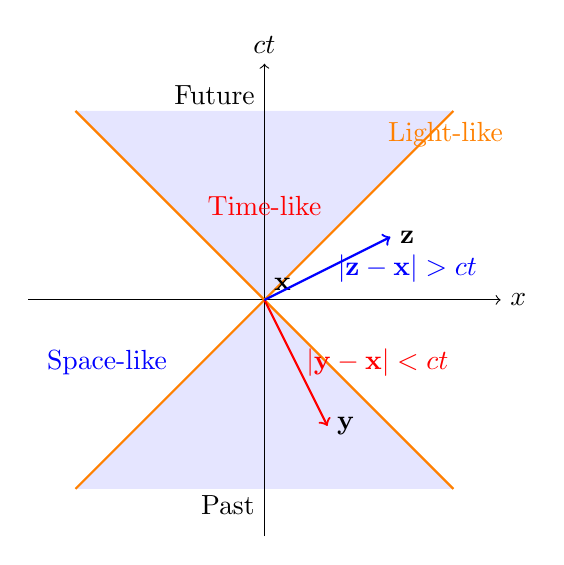
\begin{tikzpicture}[scale=2]
            % Shaded regions (light cone)
            \fill[blue!10] (-1.2,1.2) -- (1.2,1.2) -- (0,0) -- cycle; % future
            \fill[blue!10] (-1.2,-1.2) -- (1.2,-1.2) -- (0,0) -- cycle; % past

            % Axes
            \draw[->] (0,-1.5) -- (0,1.5) node[above] {$ct$};
            \draw[->] (-1.5,0) -- (1.5,0) node[right] {$x$};

            % Light cone lines
            \draw[thick,orange] (-1.2,-1.2) -- (1.2,1.2);
            \draw[thick,orange] (1.2,-1.2) -- (-1.2,1.2);

            % Labels
            \node[above right] at (0.0,0.0) {$\mathbf{x}$};
            \node[right] at (0.4,-0.8) {$\mathbf{y}$};
            \node[right] at (0.8,0.4) {$\mathbf{z}$};
            \node[left] at (0,1.3) {Future};
            \node[left] at (0,-1.3) {Past};
            \node[red] at (0,0.6) {Time-like};
            \node[blue] at (-1.0,-0.4) {Space-like};
            \node[orange] at (1.15,1.05) {Light-like};

            % Vector arrows
            \draw[->,red,thick] (0,0) -- (0.4,-0.8) node[midway,right] {$|\mathbf{y}-\mathbf{x}| < ct$};
            \draw[->,blue, thick] (0,0) -- (0.8,0.4) node[midway,right] {$|\mathbf{z}-\mathbf{x}| > ct$};
        \end{tikzpicture}
    \end{minipage}
    \hfill
    \begin{minipage}{0.45\textwidth}
        We already know that at equal times the commutator is zero for different spatial points:
        \[
            \left[\hat{O}_1(\mathbf{x}, t),\, \hat{O}_2(\mathbf{z}, t)\right] = 0, \quad \mathbf{x} \neq \mathbf{z},
        \]
        since it must be a spacelike separation \((x_\mu - z_\mu)(x^{\mu}-z^{\mu}) = 0\): a measurement at \(\mathbf{x}\) cannot influence a measurement at \(\mathbf{z}\) if they are not causally connected.

        If we recall the Heisenberg uncertainty principle, we know that two observables \(\hat{O}_1\) and \(\hat{O}_2\) can be measured simultaneously with arbitrary precision if they commute:
        \[
            \Delta O_1 \Delta O_2 \geq \frac{1}{2} \left| \langle \left[\hat{O}_1,\, \hat{O}_2\right] \rangle \right|.
        \]
    \end{minipage}
\end{figure}
If two quantities commute, they can be measured simultaneously with arbitrary precision, meaning that a measurement of one does not disturb the other. This is crucial for preserving causality in quantum field theory, as it ensures that measurements at spacelike-separated points do not influence each other. We have to check if our theory respects this prescriptions.

To answer these questions, we have to compute the commutator between two field operators at different spacetime points: let us define the \textbf{Klein-Gordon propagator} as
\[
    \Delta(x-y) = \left[\hat{\psi}(x),\, \hat{\psi}(y)\right],
\]
where \(x = (x_0,\, \mathbf{x})\) and \(y = (y_0,\, \mathbf{y})\) are two generic spacetime points. We have to check three things:
\begin{enumerate}
    \item \(\Delta(x-y)\) is Lorentz invariant;
    \item \(\Delta(x-y) \neq 0\) for \((x-y)^2 > 0\) (timelike separation);
    \item \(\Delta(x-y) = 0\) for \((x-y)^2 < 0\) (spacelike separation).
\end{enumerate}
Let us first compute the propagator, which phisically describes the amplitude for a particle created at point \(y\) to be annihilated at point \(x\):
\[
    \begin{aligned}
        \Delta(x-y) & = \left[\hat{\psi}(x),\, \hat{\psi}(y)\right] = \int \frac{\mathrm{d}^3 \mathbf{p}}{(2\pi)^3} \frac{1}{\sqrt{2\omega_{\mathbf{p}}}} \int \frac{\mathrm{d}^3 \mathbf{q}}{(2\pi)^3} \frac{1}{\sqrt{2\omega_{\mathbf{q}}}}                                                                                                                                                 \\
                    & \quad \times \left[ \hat{a}_{\mathbf{p}} e^{-i p_{\mu} x^{\mu}} + \hat{a}^{\dagger}_{\mathbf{p}} e^{i p_{\mu} x^{\mu}},\, \hat{a}_{\mathbf{q}} e^{-i q_{\mu} y^{\mu}} + \hat{a}^{\dagger}_{\mathbf{q}} e^{i q_{\mu} y^{\mu}} \right]                                                                                                                                    \\
                    & = \int \frac{\mathrm{d}^3 \mathbf{p}\mathrm{d}^3 \mathbf{q}}{(2\pi)^6} \frac{1}{2\sqrt{\omega_{\mathbf{p}} \omega_{\mathbf{q}}}} \left\{ [\hat{a}_\mathbf{p} ,\, \hat{a}^{\dagger}_\mathbf{q}]\left( e^{-i(p_{\mu}x^{\mu} - q_{\mu}y^{\mu})}\right) + [\hat{a}^{\dagger}_\mathbf{p} ,\, \hat{a}_\mathbf{q}]\left( e^{i(p_{\mu}x^{\mu} - q_{\mu}y^{\mu})}\right)\right\} \\
                    & = \int \frac{\mathrm{d}^3 \mathbf{p}\mathrm{d}^3 \mathbf{q}}{(2\pi)^3} \frac{1}{2\sqrt{\omega_{\mathbf{p}} \omega_{\mathbf{q}}}} \delta^{(3)}(\mathbf{p}-\mathbf{q}) \left(e^{-i(p_{\mu}x^{\mu} - q_{\mu}y^{\mu})} - e^{i(p_{\mu}x^{\mu} - q_{\mu}y^{\mu})}\right)                                                                                                      \\
                    & = \int \frac{\mathrm{d}^3 \mathbf{p}}{(2\pi)^3} \frac{1}{2\omega_{\mathbf{p}}} \left( e^{-i p_{\mu} (x^{\mu}-y^{\mu})} - e^{i p_{\mu} (x^{\mu}-y^{\mu})} \right),
    \end{aligned}
\]

Now we can check the three considerations:
\begin{enumerate}
    \item \textbf{Lorentz invariance}: the exponentials \(e^{\pm i p_{\mu} (x^{\mu}-y^{\mu})}\) are manifestly Lorentz invariant since they depend on the contraction of two four-vectors; the measure \(\mathrm{d}^3 \mathbf{p}/(2\pi)^3 2\omega_{\mathbf{p}}\) is Lorentz invariant, as we have previously shown at the very end of section \ref{sec:KG_particle_states}; thus the whole expression is Lorentz invariant. This means that if we compute \(\Delta(x-y)\) in a reference frame where \(x\) and \(y\) are simultaneous, the result will hold for any other spacetime events which is related to \(y\) by a Lorentz transformation. But since we cannot relate events inside and outside the light cone with a Lorentz transformation, we can chack that the commutator vanishes for only one value of \(y\) outside of \(x\) light-cone, then it will be true for events throughout the whole region.
    \item \textbf{Timelike separation}: \(\Delta(x-y) \neq 0\). Let us consider the case where \(x\) and \(y\) are separated only in time, i.e. \(\mathbf{x} = \mathbf{y}\) and \(t_x \neq t_y\), thus \((x-y)^2 > 0\). We want to prove, in the easiest case where \(x = (t,\, \mathbf{0})\) and \(y=(0, \mathbf{0})\), that the commutator do not vanish:
          \[
              \Delta(x-y) = \int \frac{\mathrm{d}^3 \mathbf{p}}{(2\pi)^3} \frac{1}{2\omega_{\mathbf{p}}} \left( e^{-i \omega_{\mathbf{p}} t} - e^{i \omega_{\mathbf{p}} t} \right).
          \]
          If we move to spherical coordinates in momentum space, we get:
          \[
              \Delta(x-y) = \frac{1}{4\pi^2} \int_0^{\infty} \mathrm{d}\vert \mathbf{p} \vert \frac{\vert \mathbf{p} \vert^2}{\sqrt{\vert \mathbf{p} \vert^2 + m^2}} \left( e^{-i \sqrt{\vert \mathbf{p} \vert^2 + m^2} t} - e^{i \sqrt{\vert \mathbf{p} \vert^2 + m^2} t} \right).
          \]
          Now we can perform a change of variable from \(\vert \mathbf{p} \vert\) to \(E_{\mathbf{p}} = \sqrt{\vert \mathbf{p} \vert^2 + m^2}\), so that \(\mathrm{d}\vert \mathbf{p} \vert = \frac{E_{\mathbf{p}}}{\sqrt{E^2_{\mathbf{p}} - m^2}} \mathrm{d}E_{\mathbf{p}}\), thus we get:
          \[
              \mathrm{d}\vert \mathbf{p} \vert \vert \mathbf{p} \vert^2 = E_{\mathbf{p}} \sqrt{E^2_{\mathbf{p}} - m^2} \mathrm{d} E_{\mathbf{p}},
          \]
          and the integral becomes
          \[
              \Delta(x-y) = \frac{1}{4\pi^2} \int_m^{\infty} \mathrm{d}E_{\mathbf{p}} \sqrt{E^2_{\mathbf{p}} - m^2} \left( e^{-i E_{\mathbf{p}} t} - e^{i E_{\mathbf{p}} t} \right).
          \]
          The solution of this integral can be computed through \textit{Bessel functions}, and the final result is:
          \[
              \Delta(x-y) = \frac{1}{4\pi^2} \int \mathrm{d}E_{\mathbf{p}} \sqrt{E^2_{\mathbf{p}} - m^2} e^{-i E_{\mathbf{p}} t} = \frac{m}{8\pi t} \left(Y_1(mt) + i J_1(mt)\right)
          \]
          where \(Y_1\) is a Bessel function of the II kind while \(J_1\) is of the I kind. Now let's take a look at the asymptotic behaviour:
          \[
              \begin{aligned}
                  J_1(x) & =       \\
                  Y_1(x) & = \dots
              \end{aligned}
          \]
          thus when we take \(t \to \infty \) we get something like \(\sin  - \cos\) so we get
          \[
              Y_1(mt) + i {J_1}(mt) \xrightarrow{t \to \infty} i \sqrt{\frac{2}{\pi m t}}e^{-imt},
          \]
          so that
          \[
              \Delta(x-y) = \left[\hat \psi(x),\, \hat \psi(y)\right] \xrightarrow{t \to \infty} \left(e^{-imt} - e^{imt}\right) \neq 0.
          \]
    \item \textbf{Spacelike separation}: \(\Delta(x-y) = 0\). Let us now consider the case where \(x\) and \(y\) are separated only in space, i.e. \(t_x = t_y\) and \(\mathbf{x} \neq \mathbf{y}\), thus \((x-y)^2 < 0\). We want to prove, in the easiest case where \(x = (t,\, \mathbf{x})\) and \(y=(t, \mathbf{y})\), that the commutator vanishes:
          \[
              \Delta(x-y) = \int \frac{\mathrm{d}^3 \mathbf{p}}{(2\pi)^3} \frac{1}{2\omega_{\mathbf{p}}} \left( e^{-i \mathbf{p} \cdot (\mathbf{x}-\mathbf{y})} - e^{i \mathbf{p} \cdot (\mathbf{x}-\mathbf{y})} \right).
          \]
          \[
              \dots \dots \dots
          \]
          since \(x_0 = y_0 = t\), only the space variables survive in the computation, and the sum of the last two integrals (performing a change of variable from \(\mathbf{p}\) to \(-\mathbf{p}\) on the second integral) we are left with two identical terms subtracted to each other, so we get \(0\). Since this guy is Lorentz invariant, we found this result true for any \((x-y)^2 = - (x-y)^2 < 0\), since the time can be different in \(x\) and \(y\), but we are speaking of spacelike vectors.
\end{enumerate}




We have proven that KG theory mathematically preserve causality (rememner that in RQMPI we looked at how there was a non zero prob of finding a particle propagating at \(v>c\)), let's check this instance phisically: the probability of finding a particle at \(v>c\) should be null.

\section{Klein Gordon Correlators}

Let us consider  particle at a spectime point \(y = (t,\,\mathbf{y})\); how do we describe it in QFT? It is an exhited state of the vacuum \(\ket{0}\), there is some kind of exhitation localized in our quantum field at the point \(y\), like a localized and quantized wave; we recreate it with a creation operator, like \(\hat a_{\mathbf{p}} \ket{0}\), but if we create a particle with definite momentum we could not possibly now its position, so we imagine a linear combination of all possible creation operators with all possible momenta: we apply the \textbf{field operator} on the vacuum
\[
    \hat \psi(y) \ket{0}.
\]
Then let's look at the probability amplitude (with a scalar product) to find it in \(x = (t,\mathbf{x})\):
\[
    D(x-y) = \bra{0} \hat \psi (x) \hat \psi (y) \ket{0}
\]
Note that it is different from RQM, where we computed \(\bra{\mathbf{x}} e^{-i \hat H t} \ket{\mathbf{y}}\) with \(\hat H = \sqrt{\vert \mathbf{p} \vert^2 + m^2}\). Lets compute the amplitude:
\[
    \begin{aligned}
        blablabla \quad pdf \quad blablabla
    \end{aligned}
\]
\(\hat a_{\mathbf{q}}\) acting on the vacuum \(\ket{0}\) is zero, but is the same to \(\hat a^{\dagger}_{\mathbf{q}}\) acting on \(\bra{0}\) (it's just the conjugate of the other); when we see a product of operators, the idea is to use commutators \(\hat a_{\mathbf{p}} \hat a^{\dagger}_{\mathbf{q}} = \left[\hat a_{\mathbf{p}}\, ,\, \hat a^{\dagger}_{\mathbf{q}}\right] + \hat a^{\dagger}_{\mathbf{q}} \hat a_{\mathbf{p}}\); thus we found this amplitude proportional of the \textbf{propagator} (the square modulus of the amplitude gives us the probability of the propagation of the particle from \(\mathbf{y}\) to \(\mathbf{x}\)).

If we evaluate this propagator for propagations outside the light cone (spacelike separation between \(x\) and \(y\), where we consider no time separation and a space separation: \(x-y = (0, \mathbf{r})\), and \(r = \vert \mathbf{r} \vert\)) this should become zero:
\[
    \begin{aligned}
        D(x-y) & =     \\
               & = pdf
    \end{aligned}
\]
if we compute the integral in \(\mathrm{d}(\cos \theta)\) we get to
\[
    D(x-y) = -\frac{i}{2(2\pi)^2 r} \left( \int_0^{\infty} \mathrm{d} \vert \mathbf{p} \vert \dots - \dots \right)
\]
we can compose the integral since we realize it's the same but with different integral domains, so
\[
    D(x-y) = -\frac{i}{2(2\pi)^2 r} \left( \int_{-\infty}^{\infty} \mathrm{d} \vert \mathbf{p} \vert \dots \right)
\]

\begin{figure}[H]
    \centering
    \begin{minipage}{0.45\textwidth}
        \centering
        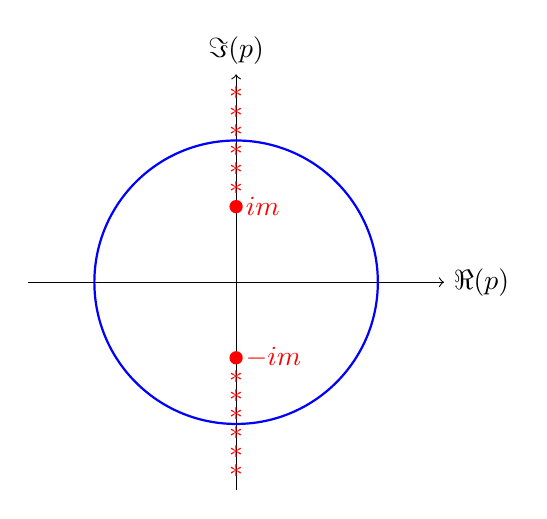
\begin{tikzpicture}[scale=1.2]
            \draw[->] (-2.2,0) -- (2.2,0) node[right] {$\Re(p)$};
            \draw[->] (0,-2.2) -- (0,2.2) node[above] {$\Im(p)$};

            \draw[thick,blue] (0,0) circle (1.5);

            \fill[red] (0.0,0.8) circle (2pt) node[right] {$im$};
            \fill[red] (0.0,-0.8) circle (2pt) node[right] {$-im$};

            \foreach \x in {1.0,1.2,1.4,1.6,1.8,2.0}{
                    \node[red] at (0,\x) {$\ast$};
                    \node[red] at (0,-\x) {$\ast$};
                }
        \end{tikzpicture}
    \end{minipage}
    \hfill
    \begin{minipage}{0.5\textwidth}
        we can now promote module \(\mathbf{p}\) to a complex variable and perform the integral with the couchy theorem; the branch cuts are as shown in figure the same as we have seen in section \ref{sec:RQM_framework}, the ones of a complex square root. We want to get the integral on the real axis, so we compute the path as an integral from \(-L\) to \(L\) on \(\mathbb{R}\) and then we take \(L \to \infty\), then we look at the contributions from the rest of the closed path
    \end{minipage}
\end{figure}

\begin{figure}[H]
    \centering
    \begin{minipage}{0.5\textwidth}
        We have then to compute the integrals on the imaginary axis as \(\vert \mathbf{p} \vert \mathrm{d} \vert \mathbf{p} \vert = -y \mathrm{d} y\) and
        \[
            D(x-y) = \dots = -\frac{1}{2 (2\pi)^2}r 2 \int_{m}^{\infty} \mathrm{d}y \, \frac{y e^{-yr}}{\sqrt{y^{2-m^2}}}.
        \]
        Now this integral is all real without problems, but is it zero?
    \end{minipage}
    \hfill
    \begin{minipage}{0.45\textwidth}
        \centering
        \begin{tikzpicture}[scale=1.1]

            \draw[->] (-2.3,0) -- (2.3,0) node[right] {$\Re(p)$};
            \draw[->] (0,-0.5) -- (0,2.5) node[above] {$\Im(p)$};

            \foreach \y in {1.0,1.2,1.4,1.6,1.8,2.0, 2.2}{
                    \node[red] at (0,\y) {$\ast$};
                }

            \draw[thick,red,<-] (0.2,0.8) arc[start angle=0,end angle=360,radius=0.2] node[right] {$C_{\epsilon}$};

            \draw[thick,->,green] (-2.2,0) -- (-1,0);
            \draw[thick,->,green] (-1,0) -- (1,0) node[below] {$C_L$};
            \draw[thick,green] (1,0) -- (2.2,0);

            \draw[thick,orange,
                postaction={decorate},
                decoration={markings, mark=at position 0.5 with {\arrow{<}}}
            ] (-2.2,0) arc[start angle=180,end angle=90,radius=2.2] node[above right] {$C_1$};

            \draw[thick,orange,
                postaction={decorate},
                decoration={markings, mark=at position 0.5 with {\arrow{>}}}
            ] (2.2,0) arc[start angle=0,end angle=90,radius=2.2] node[above left] {$C_4$};

            \draw[thick,->,blue] (0.1,2.2) -- (0.1,1.0) node[above right] {$C_2$};
            \draw[thick,<-,blue] (-0.1,2.2) -- (-0.1,1.0) node[above left] {$C_3$};

            \fill[red] (0,0.8) circle (2pt) node[right] {};
            \fill[black] (-2.2,0) circle (2pt) node[below] {$-L$};
            \fill[black] (2.2,0) circle (2pt) node[below] {$L$};

        \end{tikzpicture}
    \end{minipage}
\end{figure}

No, the exat solution is given in terms of modified bessel functions, and in the limit for \(r \sim \infty\) then \(D(x-y) \sim e^{-mr} \neq 0\) even if \(r\) is really big. but we can arrive at the same solution with approximated considerations.
This seems similar to what we obtained in RQM, but it is not: indeed if we consider the previous result
\[
    \Delta(x-y) = \left[\hat \psi(x),\, \hat \psi(y)\right] = 0
\]
for spacelike separations, so we can write
\[
    \begin{aligned}
        \Delta(x-y) & = \bra{0}\Delta(x-y)\ket{0} = \bra{0} \left[\hat \psi(x),\, \hat \psi(y)\right] \ket{0}                  \\
                    & = \bra{0} \hat \psi(x) \hat \psi(y)\ket{0} - \bra{0} \hat \psi(y) \hat \psi(x)\ket{0} = D(x-y) - D(y-x);
    \end{aligned}
\]
Note that KG theory cannot distinguish particles from antiparticles, since it does not account for charge degrees of freedom, so we can interpret this result as the probability amplitude for a particle to go from y to x minus the probability of the antiparticle going from x to y, which is an interpratation of antiparticles going backward in time to preserve the causality outside the light cone.

If we want a state in which we have a particle in the past and then in the future, we can also read this as a particle in the past, then the creation of a couple of part antipart in the future, the new particle stays in the future while the antiparticle travels backwards in time to annihilate with the initial particel. We were compiting just one half of the amplitude. All this comes from intrepretation of the athematical results of our equations. We are looking at one individual phenomenon made up by two distinct contributions.

\[
    DRAWS \, FROM \, PDF
\]
We are summing diagrams where before \(y\) and after \(x\) we have the same phenomenon, but between \(x\) and \(y\) we have in a case the particle propagating faster than light, in the other the produced antiparticle traveling backward in time faster than light only to annihilate with the other old particle in \(y\). This physical intuistion is mostly due to Feynman and his diagrams.

This kind of phenomena are called \textit{virtual phenomena}, since they cannot be measured observed, but mathematic tells us that this happens and saves our theory; even in Feynman diagrams, the virtual particle does not respect an equation of motion, there is its existence for a really brief moment, and due to uncertainty in energy etc we can justify its existence and our computing methods and interpretations.

\subsection{Green Functions}

\subsection{Feynman Propagator}